\dev{Emile Martinez}{}

\section{Généralités sur les arbres}

Un arbre est une structure de données récursives stochant hierarchiquement les données. Dans un arbres, les données sont appelées des noeuds.

\begin{definition}[arbre]
	Un arbre est un couple $(u, l)$ où $u$ est un noeud (élément) et $l$ une liste (potentiellement vide) d'arbre 
	
	\begin{itemize}[label=$\bullet$]
		\item $u$ est appelé la racine de l'arbre $(u, l)$
		
		\item si $l$ est vide, $u$ est appelé une feuille
		
		\item les arbres de $l$, sont appelés sous arbres de $(u,l)$
		
		\item Les racines des arbres de $l$ sont appelées enfant de $u$ (et ont $u$ pour parent)
		
		\item la hauteur $h(u) = h((u,l)) = 1 + \max_{A\in l} h(A)$ (et donc $1$ si $l$ est vide)
	\end{itemize}
\end{definition}

\begin{example}
	\label{10-ex1}
	$(1, \, [(2, \, []), \, (3, \, [(4,[])  (5, []), (6, [])])])$ $\qquad \longrightarrow \qquad$ \raisebox{-0.5\height}{\begin{tikzpicture}[-, node distance = 2cm]
		\node[state] (q0) {1};
		\node[state, below left of = q0] (q1) {2};
		\node[state, below right of = q0] (q2) {3};
		\node[state, below left of = q2] (q3) {4};
		\node[state, below of = q2] (q4) {5};
		\node[state, below right of = q2] (q5) {6};
		
		\draw (q0) edge[] (q1);
		\draw (q0) edge[] (q2);
		\draw (q2) edge[] (q3);
		\draw (q2) edge[] (q4);
		\draw (q2) edge[] (q5);
	\end{tikzpicture}}
\end{example}

\begin{rem}
	Il n'existe ici pas d'abre vide.
\end{rem}

\begin{example}
	L'organisation des fichiers en répertoire peut être représenté sous forme d'arbre.
\end{example}

\begin{rem}
	On peut à chaque noeud associer une étiquette. On parle alors d'arbre étiqueté.
\end{rem}

\begin{theorem}
	Identifions les arbres à des graphes non orientés où un sommet (la racine) est choisi, en considérant les liens de parentés comme des arêtes. Les arbres sont alors les graphes connexes acycliques
	\label{10-graphe}
\end{theorem}
\begin{proof}
	Exercice
\end{proof}

\begin{corollary}
	On représente les arbres comme des graphes (cf exemple \ref{10-ex1})
\end{corollary}

\begin{definition}
	Un arbre binaire est définit inductivement par :
	\begin{itemize}
		\item $E$ est un arbre vide
		\item Si $A_1$ et $A_2$ sont des arbres binaires et u une donnée, $B(u, A_1, A_2)$ est un arbre binaire, $A_1$ étant le sous-arbre gauche, et $A_2$ le droit.
	\end{itemize}
\end{definition}

\begin{idee}
	Les arbres binaires sont des arbres dont les listes sont de taille 2, mais où l'on rajoute des arbres vides.
\end{idee}

\begin{example}
	Représentation d'une expression arithmétique :\\
	\begin{minipage}{0.4 \linewidth}
		$3 \times (4 + 5)$ \\
		$\to N(\times, N(3, E, E), A)$\\
		avec $A = N(+, N(4, E, E), N(5, E, E))$
	\end{minipage} \quad $\to$ \quad \begin{minipage}{0.4\linewidth}
		\begin{tikzpicture}[-]
			\node[state] (q0) {$\times$};
			\node[state, below left = 1cm and 1.2cm of q0] (q1) {$3$};
			\node[state, below right = 1cm and 1.2cm of q0] (q2) {$+$};
			\node[below left = 1cm and 0.5cm of q1] (q3) {E};
			\node[below right = 1cm and 0.5cm of q1] (q4) {E};
			\node[state, below left = 1cm and 0.5cm of q2] (q5) {$4$};
			\node[state, below right = 1cm and 0.5cm of q2] (q6) {$5$};
			\node[below left = 1cm and 0.1cm of q5] (q7) {E};
			\node[below right = 1cm and 0.1cm of q5] (q8) {E};
			\node[below left = 1cm and 0.1cm of q6] (q9) {E};
			\node[below right = 1cm and 0.1cm of q6] (q10) {E};
			
			\draw (q0) edge[] (q1);
			\draw (q0) edge[] (q2);
			\draw (q1) edge[] (q3);
			\draw (q1) edge[] (q4);
			\draw (q2) edge[] (q5);
			\draw (q2) edge[] (q6);
			\draw (q5) edge[] (q7);
			\draw (q5) edge[] (q8);
			\draw (q6) edge[] (q9);
			\draw (q6) edge[] (q10);
		\end{tikzpicture}
	\end{minipage}
\end{example}

\section{Représentation informatique}

\subsection{Représentation comme structure inductive}

En représentant un arbre en utilisant sa structure inductive, on obtient :\begin{itemize}[label=$\bullet$]
	\item \textbf{Pour les arbres généraux}
	\begin{lstlisting}
type 'a arbre = N of 'a arb_liste and
type 'a bin arb_liste = V | Cons of (a arb *('a arb_liste));;
	\end{lstlisting}
	\item \textbf{Pour les arbres binaires}
	\begin{lstlisting}
type 'a bin = E | B of 'a * 'a bin * 'a bin;;
	\end{lstlisting}
\end{itemize}

\noindent \textbf{Développement 1 :} Correspondance entre les arbres binaires et les arbres généraux de taille $n$ et utilisation en C

\subsection{Représentation comme un graphe}

Les arbres étant des graphes connexes acycliques (cf. théorème \ref{10-graphe}), on peut les représentés comme tels :\begin{itemize}
	\item par des listes (ou dictionnaires) d'adjacence
	\item Par une matrice d'adjacence
	\item Comme la liste de toutes les arêtes
\end{itemize}

\begin{rem}
	N'exploitant pas la structure d'arbres, ces structures sont peu utilisées.
\end{rem}

\subsection{Représentation par un tableau}

SI les identifiants des noeuds sont des entiers de $0$ à $n-1$, on peut stocker l'arbre dans un tableau de taille $n$, la case $i$ contenant l'identifiant du père du noeud $i$, $-1$ si il est racine.

\begin{example}\quad
	\begin{minipage}{0.35\linewidth}
		\begin{tikzpicture}[-, node distance = 2cm]
			\node[state] (q0) {1};
			\node[state, below left of = q0] (q1) {2};
			\node[state, below of = q0] (q2) {3};
			\node[state, below right of = q0] (q3) {4};
			\node[state, below left of = q2] (q4) {5};
			\node[state, below right of = q2] (q5) {0};
			
			\draw (q0) edge[] (q1);
			\draw (q0) edge[] (q2);
			\draw (q0) edge[] (q3);
			\draw (q2) edge[] (q4);
			\draw (q2) edge[] (q5);
		\end{tikzpicture}
	\end{minipage}
	\begin{minipage}{0.45\linewidth}
		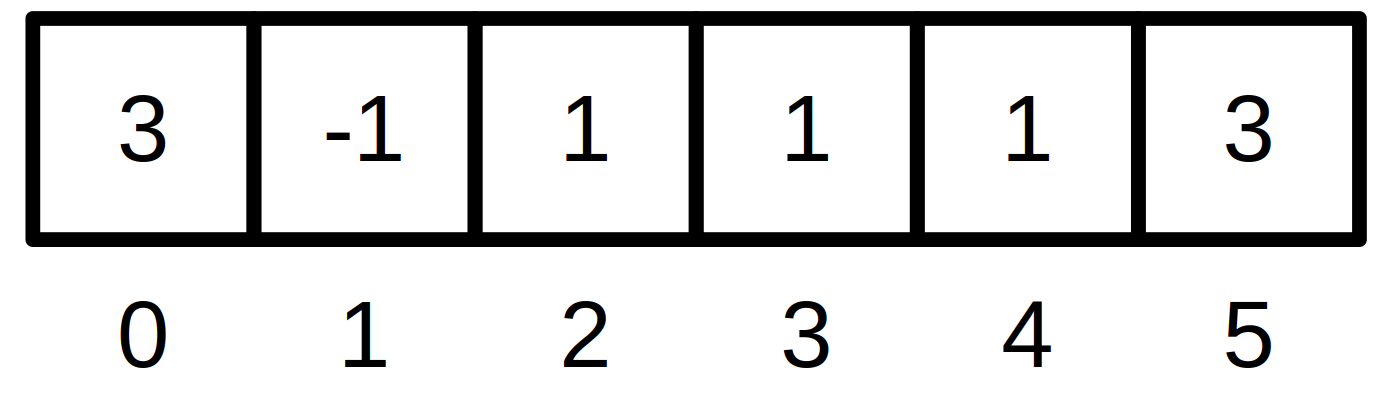
\includegraphics[width=0.9\linewidth]{lecon/10-arbres/arbre-tableau.png}
	\end{minipage}
\end{example}

\begin{rem}
	On ne stocke ici que la structure. Pour stocker des données, on produit un tableau de couples.
\end{rem}

\subsection{Représentation d'un arbre binaire presque complet}

\begin{definition}[Arbre binaire presque complet] \enspace\\
	\begin{minipage}{0.6\linewidth}
		Un arbre binaire presque complet est un arbre binaire dont tous les étages sont remplies sauf éventuellement le dernier qui est alors rempli à gauche
	\end{minipage} \qquad \begin{minipage}{0.4\linewidth}
		\begin{tikzpicture}[-]
			\node[state, scale=0.3] (q0) {};
			\node[state, scale=0.3, below left = 0.25 cm and 0.8cm of q0] (q1) {};
			\node[state, scale=0.3, below right = 0.25 cm and 0.8cm of q0] (q2) {};
			\node[state, scale=0.3, below left = 0.25 cm and 0.4cm of q1] (q3) {};
			\node[state, scale=0.3, below right = 0.25 cm and 0.4cm of q1] (q4) {};
			\node[state, scale=0.3, below left = 0.25 cm and 0.4cm of q2] (q5) {};
			\node[state, scale=0.3, below right = 0.25 cm and 0.4cm of q2] (q6) {};
			\node[state, scale=0.3, below left = 0.25 cm and 0.1cm of q3] (q7) {};
			\node[state, scale=0.3, below right = 0.25 cm and 0.1cm of q3] (q8) {};
			\node[state, scale=0.3, below left = 0.25 cm and 0.1cm of q4] (q9) {};
			
			\draw (q0) edge[] (q1);
			\draw (q0) edge[] (q2);
			\draw (q1) edge[] (q3);
			\draw (q1) edge[] (q4);
			\draw (q2) edge[] (q5);
			\draw (q2) edge[] (q6);
			\draw (q3) edge[] (q7);
			\draw (q3) edge[] (q8);
			\draw (q4) edge[] (q9);
		\end{tikzpicture}
	\end{minipage}
\end{definition}

\begin{minipage}{0.45\linewidth}
	\begin{principe}
		On peut alors représenter un tas par un tableau. On numérote alors les sommets ci contre, donnant l'indice dans le tableau. Les fils du noeuds d'indice $i$ se retrouve aux cases $2\times i+1$, $2\times i+2$, et son père $\left\lfloor \dfrac{i-1}{2}\right\rfloor$
	\end{principe}
\end{minipage}
\qquad
\begin{minipage}{0.45\linewidth}
	\begin{tikzpicture}[-]
		\node[state, scale=0.4] (q0) {};
		\node[state, scale=0.4, below left = 0.55 cm and 1.1cm of q0] (q1) {};
		\node[state, scale=0.4, below right = 0.55 cm and 1.1cm of q0] (q2) {};
		\node[state, scale=0.4, below left = 0.55 cm and 0.6cm of q1] (q3) {};
		\node[state, scale=0.4, below right = 0.55 cm and 0.6cm of q1] (q4) {};
		\node[state, scale=0.4, below left = 0.55 cm and 0.6cm of q2] (q5) {};
		\node[state, scale=0.4, below right = 0.55 cm and 0.6cm of q2] (q6) {};
		\node[state, scale=0.4, below left = 0.55 cm and 0.2cm of q3] (q7) {};
		\node[state, scale=0.4, below right = 0.55 cm and 0.2cm of q3] (q8) {};
		\node[state, scale=0.4, below left = 0.55 cm and 0.2cm of q4] (q9) {};
		
		\node[above right = 0cm and 0cm of q0] (l0) {\textcolor{cyan}{0}};
		\node[above left = 0cm and 0cm of q1] (l1) {\textcolor{cyan}{1}};
		\node[above right = 0cm and 0cm of q2] (l2) {\textcolor{cyan}{2}};
		\node[above left = 0cm and 0cm of q3] (l3) {\textcolor{cyan}{3}};
		\node[above right = 0cm and 0cm of q4] (l4) {\textcolor{cyan}{4}};
		\node[below = 0cm of q5] (l5) {\textcolor{cyan}{5}};
		\node[above right = 0cm and 0cm of q6] (l6) {\textcolor{cyan}{6}};
		\node[below = 0cm of q7] (l7) {\textcolor{cyan}{7}};
		\node[below = 0cm of q8] (l8) {\textcolor{cyan}{8}};
		\node[below = 0cm of q9] (l9) {\textcolor{cyan}{9}};
		
		\draw (q0) edge[] (q1);
		\draw (q0) edge[] (q2);
		\draw (q1) edge[] (q3);
		\draw (q1) edge[] (q4);
		\draw (q2) edge[] (q5);
		\draw (q2) edge[] (q6);
		\draw (q3) edge[] (q7);
		\draw (q3) edge[] (q8);
		\draw (q4) edge[] (q9);
	\end{tikzpicture}
\end{minipage}\\

\begin{example}\enspace\\
	\begin{minipage}{0.5\linewidth}
		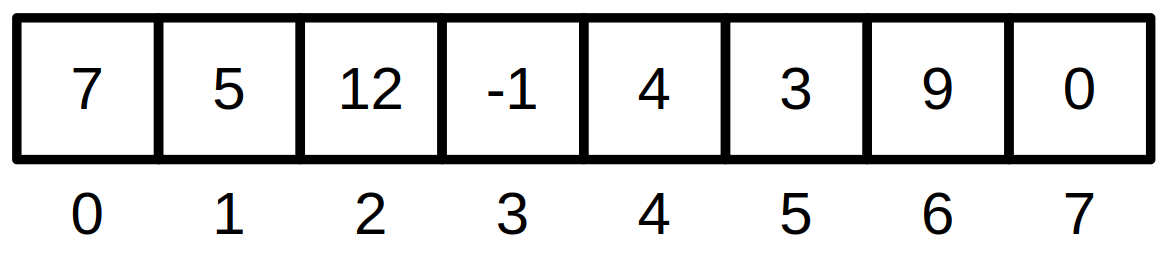
\includegraphics[width=\linewidth]{lecon/10-arbres/semi-complet.png}
	\end{minipage} \qquad
	\begin{minipage}{0.5\linewidth}
		\begin{tikzpicture}[-]
			\node[state] (q0) {7};
			\node[state, below left = 0.55 cm and 1.1cm of q0] (q1) {5};
			\node[state, below right = 0.55 cm and 1.1cm of q0] (q2) {12};
			\node[state, below left = 0.55 cm and 0.4cm of q1] (q3) {-1};
			\node[state, below right = 0.55 cm and 0.4cm of q1] (q4) {4};
			\node[state, below left = 0.55 cm and 0.4cm of q2] (q5) {3};
			\node[state, below right = 0.55 cm and 0.4cm of q2] (q6) {9};
			\node[state, below left = 0.55 cm and 0.2cm of q3] (q7) {0};
			
			\node[above right = 0cm and 0cm of q0] (l0) {\textcolor{cyan}{0}};
			\node[above left = 0cm and 0cm of q1] (l1) {\textcolor{cyan}{1}};
			\node[above right = 0cm and 0cm of q2] (l2) {\textcolor{cyan}{2}};
			\node[above left = 0cm and 0cm of q3] (l3) {\textcolor{cyan}{3}};
			\node[above right = 0cm and 0cm of q4] (l4) {\textcolor{cyan}{4}};
			\node[below = 0cm of q5] (l5) {\textcolor{cyan}{5}};
			\node[above right = 0cm and 0cm of q6] (l6) {\textcolor{cyan}{6}};
			\node[below = 0cm of q7] (l7) {\textcolor{cyan}{7}};
			
			\draw (q0) edge[] (q1);
			\draw (q0) edge[] (q2);
			\draw (q1) edge[] (q3);
			\draw (q1) edge[] (q4);
			\draw (q2) edge[] (q5);
			\draw (q2) edge[] (q6);
		\draw (q3) edge[] (q7);
		\end{tikzpicture}
	\end{minipage}
\end{example}

\section{Application}

\begin{com}
	A chaque fois on va écrire en début quelle représentation on utilise pour notre application. Néanmoins, en classe, on pourrait le laisser proposer par les élèves (une fois l'application présentée). On justifie de ce fait notre organisation, ou les applications arrivent toutes ensembles à la fin. (mais on écrit quand même la représentation au début pour que ce soit plus facile de naviguer à la partie que l'on souhaite).
\end{com}

\subsection{Dictionnaires}

\noindent \textbf{Représentation :} Structure inductive

\begin{definition}
	Un arbre binaire de recherche $N(x, G, D)$ est un arbre binaire de recherche (ABR) si $G$ et $D$ sont des ABR et si, selon un attribut $a$, $\max\limits_{u\in G} u.a\leq x.a \leq \min\limits_{v\in D} v.a$ (avec $E$ qui est un ABR et $\max\limits_{u\in E} u.a = -\infty$ et $\min\limits_{u \in E} u.a = +\infty$)
\end{definition}

\begin{proposition}
	Chercher et insérer dans un ABR est en $O(h)$
\end{proposition}

\begin{proposition}
	En imposant des contraintes supplémentaires (exemple arbres rouge-noir), on peut forcer $h = O(\log n)$
\end{proposition}

\begin{definition}
	Un dictionnaire (ou tableau associatif) est un tableau où les indices (clés) ne se limite pas à $\llbracket 0, n\rrbracket$
\end{definition}

\begin{idee}
	On peut alors implémenter un dictionnaire par un ABR, les clés étant les étiquettes des nœuds, à condition d'avoir un ordre total sur les clés
\end{idee}

\begin{theorem}
	Une implémentation efficace des dictionnaires par ABR permet des opérations de base en $O(\log n)$
\end{theorem}

\begin{com}
	Si on ne veut pas faire le développement 2, et qu'on préfère celui sur les arbres k-dimensionnel, on peut aussi parler aussi du pb des k-plus proches voisins et parler des ABR comme des arbres k-dim pour résoudre le pb
\end{com}

\subsection{Classes d'équivalence}

\noindent \textbf{Représentation :} Tableaux

\begin{definition}
	Une structure union \& trouver est une structure implémentant les classes d'équivalence, permettant de trouver les représentants d'une classe et d'unir deux classes.
\end{definition}

\begin{idee}
	On implémente cette structure sous formes d'un ensemble d'arbres (forêt), où chaque arbre représente une classe et où la racine est le représentant de la classe
\end{idee}

\begin{example}
	La relation d'égalité modulo 3 sur $\llbracket 0, 7 \rrbracket$ peut être représenté par : \\
	\begin{minipage}{0.4\linewidth}
		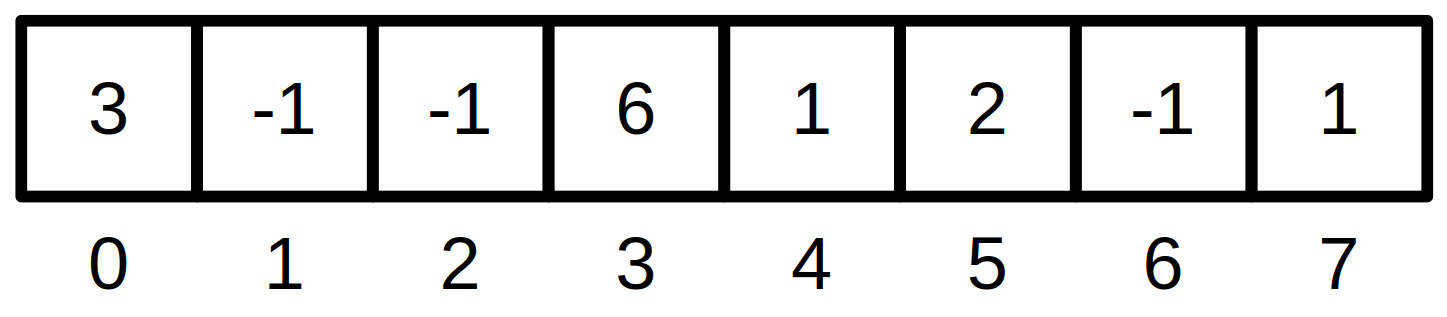
\includegraphics[width=\linewidth]{lecon/10-arbres/classe_equiv.png}
	\end{minipage}
	\qquad
 	\begin{minipage}{0.4\linewidth}
 		\begin{tikzpicture}[->, node distance=2cm]
 			\node[state] (q0) {$1$};
 			\node[state, below left of = q0] (q1) {$4$};
 			\node[state, below right of = q0] (q2) {$7$};	
 			\node[state, right = 2.5cm of q0] (q3) {$2$};
 			\node[state, below of = q3] (q4) {$5$};
 			\node[state, above right = 0.2cm and 2cm of q3] (q5) {$6$};
 			\node[state, below of = q5] (q6) {$3$};
 			\node[state, below of = q6] (q7) {$0$};
 			
 			\draw (q0) edge[] (q1);
 			\draw (q0) edge[] (q2);
 			\draw (q3) edge[] (q4);
 			\draw (q5) edge[] (q6);
 			\draw (q6) edge[] (q7);
 		\end{tikzpicture}
 	\end{minipage}
\end{example}

\begin{proposition}
	Si on unifie en faisant pointer la racine de l'arbre le moins profond vers celle de l'arbre le plus profond, on obtient des opérations unir et trouver en $O(\log(n))$
\end{proposition}

\subsection{Arbres couvrant de poids minimal}

\noindent \textbf{Représentation :} liste des arêtes

\begin{definition}
	Dans un graphe pondéré connexe, un arbre couvrant de poids minimal, est un sous-ensemble maximal d'arêtes sans cycles de somme de poids minimal.
\end{definition}

\begin{algorithm}[H]
	\caption{$Kruskal(L)$}
	\Entree{$L$ liste des arêtes}
	\Sortie{Liste des arêtes d'un ACM}
	$L\gets L$ trié\\
	$res \gets []$\\
	\Pour{$a$ parcourant $L$}
	{
		\Si{$a$ ne rajoute pas de cycle dans $res$}
		{
			Ajouter $a$ à $res$
		}
	}
	\Retour{$res$}
\end{algorithm}

\begin{proposition}
	En implémentant la détection de cycle par une structure union \& trouver, Kruskal renvoie un arbre couvrant de poids minimal en $O(|L| \times \log |L|)$
\end{proposition}

\subsection{Files de priorité}

\noindent \textbf{Représentation :} celles des arbres semi-complet

\begin{definition}
	Une file de priorité est une séquence de données dont on peut extraire la donnée d'attribut minimum, et rajouter des données.
\end{definition}

\begin{idee}
	On peut implémenter les files de priorité par des tas min
\end{idee}

\begin{definition}
	Un tas min est un arbre semi-complet où chaque noeud a un attribut plus petit que ses fils
\end{definition}

\noindent \textbf{Développement 2 :} Correction de l'insertion dans un tas min et discussion sur l'implémentation

\begin{principe}
	\enspace
	\begin{itemize}[label=$\star$]
		\item Pour ajouter un élément, on le met au bout du tablea et on l'échange avec son père tant qu'il est plus petit
		\item, Pour extraire le min, on met le dernier élément du tableau au début et on l'inverse avec le plus petit de ses fils tant qu'il est plus grand.
	\end{itemize}
\end{principe}

\begin{proposition}
	Cette implémentation permet des opérations en $O(\log n)$
\end{proposition}

\begin{appl}
	Trier par tas en $O(n \log n)$
\end{appl}